\documentclass[1p]{elsarticle_modified}
%\bibliographystyle{elsarticle-num}

%\usepackage[colorlinks]{hyperref}
%\usepackage{abbrmath_seonhwa} %\Abb, \Ascr, \Acal ,\Abf, \Afrak
\usepackage{amsfonts}
\usepackage{amssymb}
\usepackage{amsmath}
\usepackage{amsthm}
\usepackage{scalefnt}
\usepackage{amsbsy}
\usepackage{kotex}
\usepackage{caption}
\usepackage{subfig}
\usepackage{color}
\usepackage{graphicx}
\usepackage{xcolor} %% white, black, red, green, blue, cyan, magenta, yellow
\usepackage{float}
\usepackage{setspace}
\usepackage{hyperref}

\usepackage{tikz}
\usetikzlibrary{arrows}

\usepackage{multirow}
\usepackage{array} % fixed length table
\usepackage{hhline}

%%%%%%%%%%%%%%%%%%%%%
\makeatletter
\renewcommand*\env@matrix[1][\arraystretch]{%
	\edef\arraystretch{#1}%
	\hskip -\arraycolsep
	\let\@ifnextchar\new@ifnextchar
	\array{*\c@MaxMatrixCols c}}
\makeatother %https://tex.stackexchange.com/questions/14071/how-can-i-increase-the-line-spacing-in-a-matrix
%%%%%%%%%%%%%%%

\usepackage[normalem]{ulem}

\newcommand{\msout}[1]{\ifmmode\text{\sout{\ensuremath{#1}}}\else\sout{#1}\fi}
%SOURCE: \msout is \stkout macro in https://tex.stackexchange.com/questions/20609/strikeout-in-math-mode

\newcommand{\cancel}[1]{
	\ifmmode
	{\color{red}\msout{#1}}
	\else
	{\color{red}\sout{#1}}
	\fi
}

\newcommand{\add}[1]{
	{\color{blue}\uwave{#1}}
}

\newcommand{\replace}[2]{
	\ifmmode
	{\color{red}\msout{#1}}{\color{blue}\uwave{#2}}
	\else
	{\color{red}\sout{#1}}{\color{blue}\uwave{#2}}
	\fi
}

\newcommand{\Sol}{\mathcal{S}} %segment
\newcommand{\D}{D} %diagram
\newcommand{\A}{\mathcal{A}} %arc


%%%%%%%%%%%%%%%%%%%%%%%%%%%%%5 test

\def\sl{\operatorname{\textup{SL}}(2,\Cbb)}
\def\psl{\operatorname{\textup{PSL}}(2,\Cbb)}
\def\quan{\mkern 1mu \triangleright \mkern 1mu}

\theoremstyle{definition}
\newtheorem{thm}{Theorem}[section]
\newtheorem{prop}[thm]{Proposition}
\newtheorem{lem}[thm]{Lemma}
\newtheorem{ques}[thm]{Question}
\newtheorem{cor}[thm]{Corollary}
\newtheorem{defn}[thm]{Definition}
\newtheorem{exam}[thm]{Example}
\newtheorem{rmk}[thm]{Remark}
\newtheorem{alg}[thm]{Algorithm}

\newcommand{\I}{\sqrt{-1}}
\begin{document}

%\begin{frontmatter}
%
%\title{Boundary parabolic representations of knots up to 8 crossings}
%
%%% Group authors per affiliation:
%\author{Yunhi Cho} 
%\address{Department of Mathematics, University of Seoul, Seoul, Korea}
%\ead{yhcho@uos.ac.kr}
%
%
%\author{Seonhwa Kim} %\fnref{s_kim}}
%\address{Center for Geometry and Physics, Institute for Basic Science, Pohang, 37673, Korea}
%\ead{ryeona17@ibs.re.kr}
%
%\author{Hyuk Kim}
%\address{Department of Mathematical Sciences, Seoul National University, Seoul 08826, Korea}
%\ead{hyukkim@snu.ac.kr}
%
%\author{Seokbeom Yoon}
%\address{Department of Mathematical Sciences, Seoul National University, Seoul, 08826,  Korea}
%\ead{sbyoon15@snu.ac.kr}
%
%\begin{abstract}
%We find all boundary parabolic representation of knots up to 8 crossings.
%
%\end{abstract}
%\begin{keyword}
%    \MSC[2010] 57M25 
%\end{keyword}
%
%\end{frontmatter}

%\linenumbers
%\tableofcontents
%
\newcommand\colored[1]{\textcolor{white}{\rule[-0.35ex]{0.8em}{1.4ex}}\kern-0.8em\color{red} #1}%
%\newcommand\colored[1]{\textcolor{white}{ #1}\kern-2.17ex	\textcolor{white}{ #1}\kern-1.81ex	\textcolor{white}{ #1}\kern-2.15ex\color{red}#1	}

{\Large $\underline{12a_{1099}~(K12a_{1099})}$}

\setlength{\tabcolsep}{10pt}
\renewcommand{\arraystretch}{1.6}
\vspace{1cm}\begin{tabular}{m{100pt}>{\centering\arraybackslash}m{274pt}}
\multirow{5}{120pt}{
	\centering
	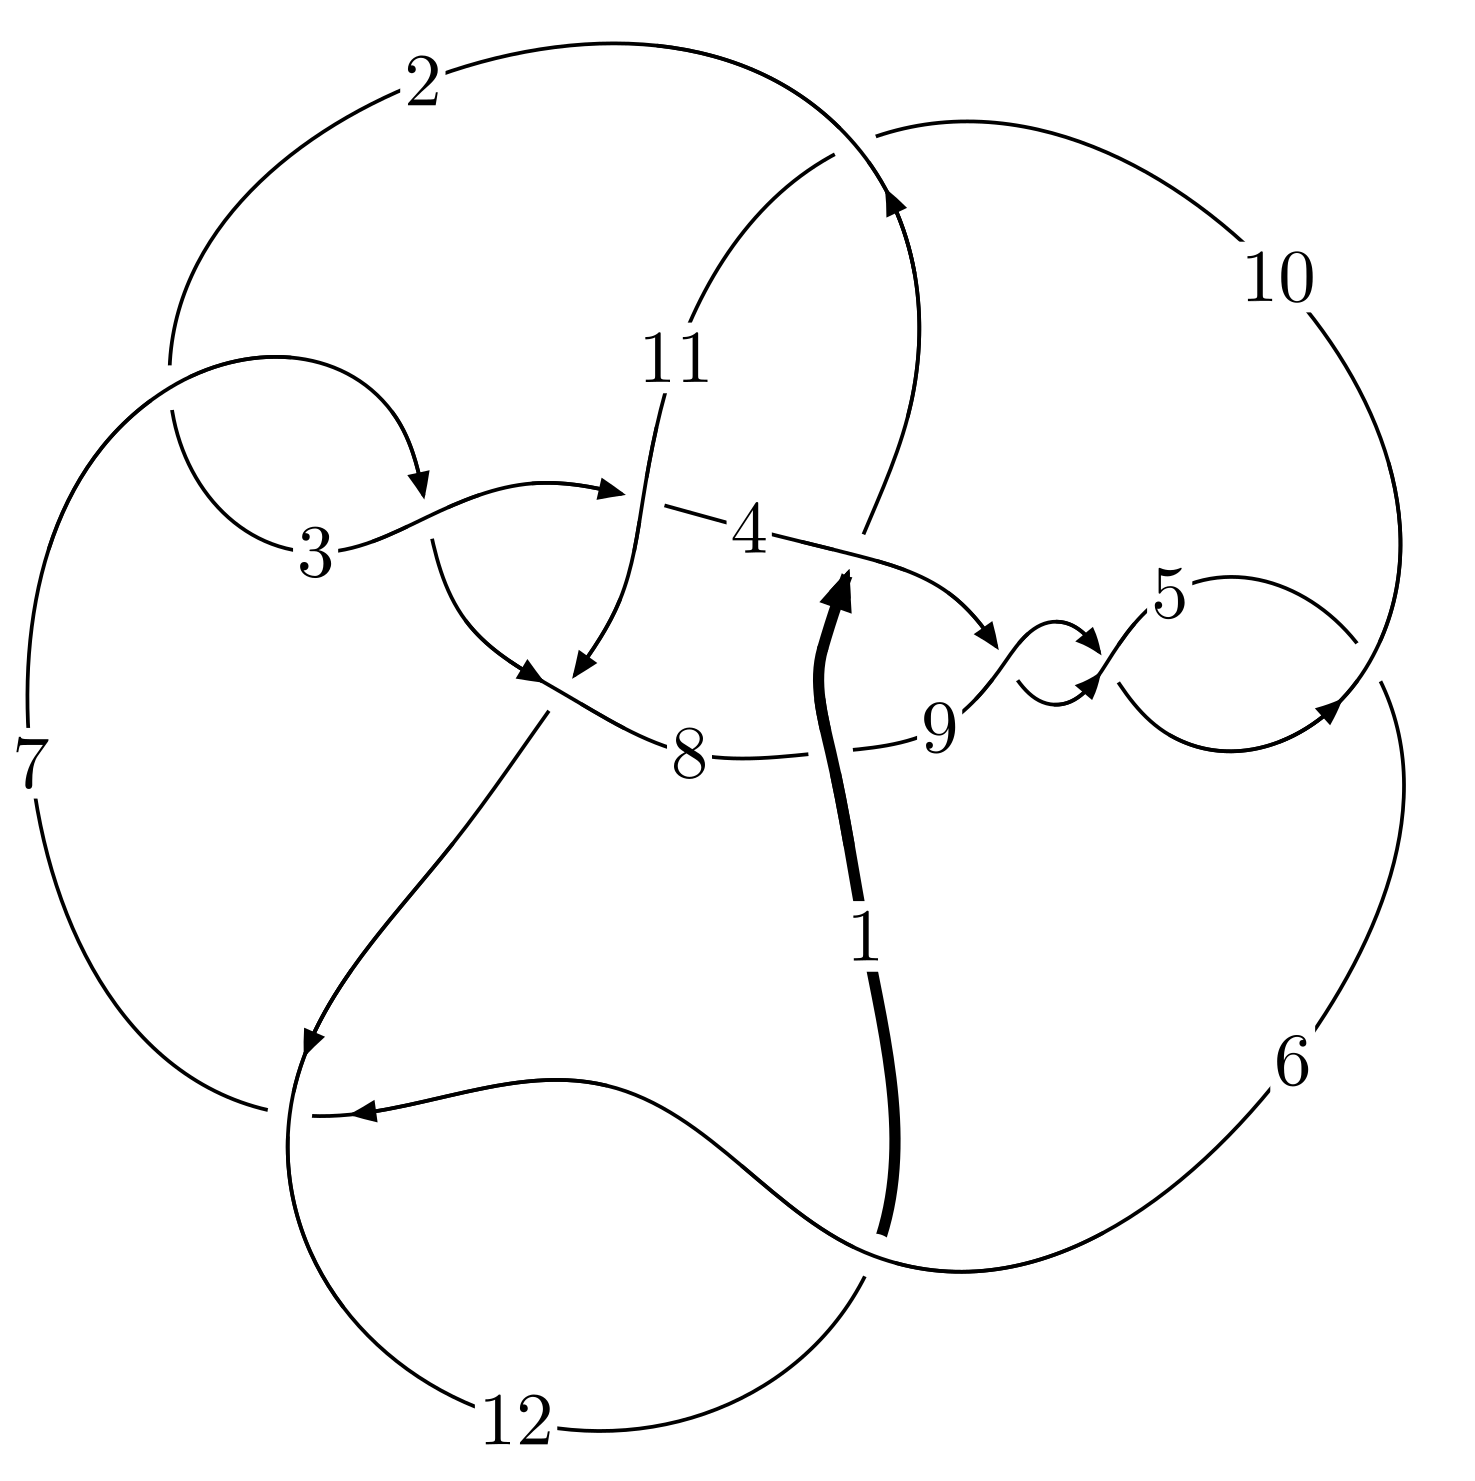
\includegraphics[width=112pt]{../../../GIT/diagram.site/Diagrams/png/1900_12a_1099.png}\\
\ \ \ A knot diagram\footnotemark}&
\allowdisplaybreaks
\textbf{Linearized knot diagam} \\
\cline{2-2}
 &
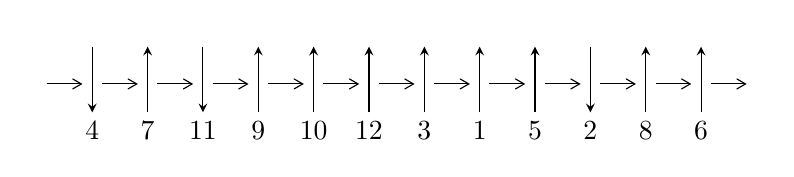
\begin{tikzpicture}[x=20pt, y=17pt]
	% nodes
	\node (C0) at (0, 0) {};
	\node (C1) at (1, 0) {};
	\node (C1U) at (1, +1) {};
	\node (C1D) at (1, -1) {4};

	\node (C2) at (2, 0) {};
	\node (C2U) at (2, +1) {};
	\node (C2D) at (2, -1) {7};

	\node (C3) at (3, 0) {};
	\node (C3U) at (3, +1) {};
	\node (C3D) at (3, -1) {11};

	\node (C4) at (4, 0) {};
	\node (C4U) at (4, +1) {};
	\node (C4D) at (4, -1) {9};

	\node (C5) at (5, 0) {};
	\node (C5U) at (5, +1) {};
	\node (C5D) at (5, -1) {10};

	\node (C6) at (6, 0) {};
	\node (C6U) at (6, +1) {};
	\node (C6D) at (6, -1) {12};

	\node (C7) at (7, 0) {};
	\node (C7U) at (7, +1) {};
	\node (C7D) at (7, -1) {3};

	\node (C8) at (8, 0) {};
	\node (C8U) at (8, +1) {};
	\node (C8D) at (8, -1) {1};

	\node (C9) at (9, 0) {};
	\node (C9U) at (9, +1) {};
	\node (C9D) at (9, -1) {5};

	\node (C10) at (10, 0) {};
	\node (C10U) at (10, +1) {};
	\node (C10D) at (10, -1) {2};

	\node (C11) at (11, 0) {};
	\node (C11U) at (11, +1) {};
	\node (C11D) at (11, -1) {8};

	\node (C12) at (12, 0) {};
	\node (C12U) at (12, +1) {};
	\node (C12D) at (12, -1) {6};
	\node (C13) at (13, 0) {};

	% arrows
	\draw[->,>={angle 60}]
	(C0) edge (C1) (C1) edge (C2) (C2) edge (C3) (C3) edge (C4) (C4) edge (C5) (C5) edge (C6) (C6) edge (C7) (C7) edge (C8) (C8) edge (C9) (C9) edge (C10) (C10) edge (C11) (C11) edge (C12) (C12) edge (C13) ;	\draw[->,>=stealth]
	(C1U) edge (C1D) (C2D) edge (C2U) (C3U) edge (C3D) (C4D) edge (C4U) (C5D) edge (C5U) (C6D) edge (C6U) (C7D) edge (C7U) (C8D) edge (C8U) (C9D) edge (C9U) (C10U) edge (C10D) (C11D) edge (C11U) (C12D) edge (C12U) ;
	\end{tikzpicture} \\
\hhline{~~} \\& 
\textbf{Solving Sequence} \\ \cline{2-2} 
 &
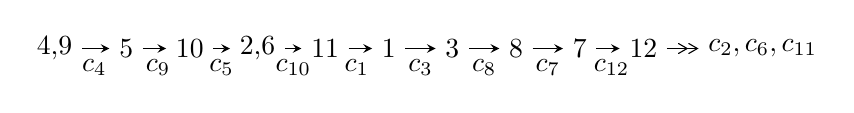
\begin{tikzpicture}[x=23pt, y=7pt]
	% node
	\node (A0) at (-1/8, 0) {4,9};
	\node (A1) at (1, 0) {5};
	\node (A2) at (2, 0) {10};
	\node (A3) at (49/16, 0) {2,6};
	\node (A4) at (33/8, 0) {11};
	\node (A5) at (41/8, 0) {1};
	\node (A6) at (49/8, 0) {3};
	\node (A7) at (57/8, 0) {8};
	\node (A8) at (65/8, 0) {7};
	\node (A9) at (73/8, 0) {12};
	\node (C1) at (1/2, -1) {$c_{4}$};
	\node (C2) at (3/2, -1) {$c_{9}$};
	\node (C3) at (5/2, -1) {$c_{5}$};
	\node (C4) at (29/8, -1) {$c_{10}$};
	\node (C5) at (37/8, -1) {$c_{1}$};
	\node (C6) at (45/8, -1) {$c_{3}$};
	\node (C7) at (53/8, -1) {$c_{8}$};
	\node (C8) at (61/8, -1) {$c_{7}$};
	\node (C9) at (69/8, -1) {$c_{12}$};
	\node (A10) at (11, 0) {$c_{2},c_{6},c_{11}$};

	% edge
	\draw[->,>=stealth]	
	(A0) edge (A1) (A1) edge (A2) (A2) edge (A3) (A3) edge (A4) (A4) edge (A5) (A5) edge (A6) (A6) edge (A7) (A7) edge (A8) (A8) edge (A9) ;
	\draw[->>,>={angle 60}]	
	(A9) edge (A10);
\end{tikzpicture} \\ 

\end{tabular} \\

\footnotetext{
The image of knot diagram is generated by the software ``\textbf{Draw programme}" developed by Andrew Bartholomew(\url{http://www.layer8.co.uk/maths/draw/index.htm\#Running-draw}), where we modified some parts for our purpose(\url{https://github.com/CATsTAILs/LinksPainter}).
}\phantom \\ \newline 
\centering \textbf{Ideals for irreducible components\footnotemark of $X_{\text{par}}$} 
 
\begin{align*}
I^u_{1}&=\langle 
7.06785\times10^{400} u^{139}-6.39249\times10^{400} u^{138}+\cdots+5.00007\times10^{401} b-3.90002\times10^{402},\\
\phantom{I^u_{1}}&\phantom{= \langle  }3.38612\times10^{403} u^{139}-2.31085\times10^{403} u^{138}+\cdots+2.35003\times10^{403} a-1.04980\times10^{405},\\
\phantom{I^u_{1}}&\phantom{= \langle  }u^{140}-2 u^{139}+\cdots-246 u+47\rangle \\
I^u_{2}&=\langle 
-127505400578 u^{31}-68289128546 u^{30}+\cdots+7817930129 b+241878697278,\\
\phantom{I^u_{2}}&\phantom{= \langle  }395700422218 u^{31}+217822084997 u^{30}+\cdots+7817930129 a-830847543053,\\
\phantom{I^u_{2}}&\phantom{= \langle  }u^{32}+u^{31}+\cdots-4 u-1\rangle \\
\\
\end{align*}
\raggedright * 2 irreducible components of $\dim_{\mathbb{C}}=0$, with total 172 representations.\\
\footnotetext{All coefficients of polynomials are rational numbers. But the coefficients are sometimes approximated in decimal forms when there is not enough margin.}
\newpage
\renewcommand{\arraystretch}{1}
\centering \section*{I. $I^u_{1}= \langle 7.07\times10^{400} u^{139}-6.39\times10^{400} u^{138}+\cdots+5.00\times10^{401} b-3.90\times10^{402},\;3.39\times10^{403} u^{139}-2.31\times10^{403} u^{138}+\cdots+2.35\times10^{403} a-1.05\times10^{405},\;u^{140}-2 u^{139}+\cdots-246 u+47 \rangle$}
\flushleft \textbf{(i) Arc colorings}\\
\begin{tabular}{m{7pt} m{180pt} m{7pt} m{180pt} }
\flushright $a_{4}=$&$\begin{pmatrix}1\\0\end{pmatrix}$ \\
\flushright $a_{9}=$&$\begin{pmatrix}0\\u\end{pmatrix}$ \\
\flushright $a_{5}=$&$\begin{pmatrix}1\\- u^2\end{pmatrix}$ \\
\flushright $a_{10}=$&$\begin{pmatrix}u\\- u^3+u\end{pmatrix}$ \\
\flushright $a_{2}=$&$\begin{pmatrix}-1.44088 u^{139}+0.983325 u^{138}+\cdots-188.804 u+44.6719\\-0.141355 u^{139}+0.127848 u^{138}+\cdots-35.9278 u+7.79995\end{pmatrix}$ \\
\flushright $a_{6}=$&$\begin{pmatrix}- u^2+1\\u^4-2 u^2\end{pmatrix}$ \\
\flushright $a_{11}=$&$\begin{pmatrix}0.252221 u^{139}-0.0372281 u^{138}+\cdots+55.2224 u-14.9395\\-0.708542 u^{139}+0.533693 u^{138}+\cdots-129.532 u+28.6376\end{pmatrix}$ \\
\flushright $a_{1}=$&$\begin{pmatrix}-1.58224 u^{139}+1.11117 u^{138}+\cdots-224.732 u+52.4718\\-0.141355 u^{139}+0.127848 u^{138}+\cdots-35.9278 u+7.79995\end{pmatrix}$ \\
\flushright $a_{3}=$&$\begin{pmatrix}-1.39386 u^{139}+1.08276 u^{138}+\cdots-289.087 u+57.6497\\-0.368782 u^{139}+0.167318 u^{138}+\cdots-50.8918 u+14.4164\end{pmatrix}$ \\
\flushright $a_{8}=$&$\begin{pmatrix}0.639687 u^{139}-0.546845 u^{138}+\cdots+104.172 u-29.0524\\0.546644 u^{139}-0.394692 u^{138}+\cdots+89.2529 u-20.5778\end{pmatrix}$ \\
\flushright $a_{7}=$&$\begin{pmatrix}0.431121 u^{139}-0.397893 u^{138}+\cdots+23.7312 u-14.0691\\0.295541 u^{139}-0.164193 u^{138}+\cdots+69.0106 u-12.1486\end{pmatrix}$ \\
\flushright $a_{12}=$&$\begin{pmatrix}-2.16500 u^{139}+1.50927 u^{138}+\cdots-300.819 u+69.7943\\-0.541777 u^{139}+0.389400 u^{138}+\cdots-99.1346 u+21.8711\end{pmatrix}$\\&\end{tabular}
\flushleft \textbf{(ii) Obstruction class $= -1$}\\~\\
\flushleft \textbf{(iii) Cusp Shapes $= 2.64192 u^{139}+5.61201 u^{138}+\cdots+1506.14 u-276.960$}\\~\\
\newpage\renewcommand{\arraystretch}{1}
\flushleft \textbf{(iv) u-Polynomials at the component}\newline \\
\begin{tabular}{m{50pt}|m{274pt}}
Crossings & \hspace{64pt}u-Polynomials at each crossing \\
\hline $$\begin{aligned}c_{1}\end{aligned}$$&$\begin{aligned}
&u^{140}-21 u^{139}+\cdots+2161255 u-89729
\end{aligned}$\\
\hline $$\begin{aligned}c_{2},c_{7}\end{aligned}$$&$\begin{aligned}
&u^{140}-38 u^{138}+\cdots+756 u+328
\end{aligned}$\\
\hline $$\begin{aligned}c_{3}\end{aligned}$$&$\begin{aligned}
&u^{140}-13 u^{139}+\cdots-20208 u-28951
\end{aligned}$\\
\hline $$\begin{aligned}c_{4},c_{5},c_{9}\end{aligned}$$&$\begin{aligned}
&u^{140}+2 u^{139}+\cdots+246 u+47
\end{aligned}$\\
\hline $$\begin{aligned}c_{6},c_{12}\end{aligned}$$&$\begin{aligned}
&u^{140}+15 u^{139}+\cdots-2958456 u-205039
\end{aligned}$\\
\hline $$\begin{aligned}c_{8}\end{aligned}$$&$\begin{aligned}
&u^{140}-7 u^{138}+\cdots+704512 u-32768
\end{aligned}$\\
\hline $$\begin{aligned}c_{10}\end{aligned}$$&$\begin{aligned}
&u^{140}+3 u^{139}+\cdots-58207 u+11101
\end{aligned}$\\
\hline $$\begin{aligned}c_{11}\end{aligned}$$&$\begin{aligned}
&u^{140}-3 u^{139}+\cdots-560200 u+26759
\end{aligned}$\\
\hline
\end{tabular}\\~\\
\newpage\renewcommand{\arraystretch}{1}
\flushleft \textbf{(v) Riley Polynomials at the component}\newline \\
\begin{tabular}{m{50pt}|m{274pt}}
Crossings & \hspace{64pt}Riley Polynomials at each crossing \\
\hline $$\begin{aligned}c_{1}\end{aligned}$$&$\begin{aligned}
&y^{140}-125 y^{139}+\cdots-1146758776985 y+8051293441
\end{aligned}$\\
\hline $$\begin{aligned}c_{2},c_{7}\end{aligned}$$&$\begin{aligned}
&y^{140}-76 y^{139}+\cdots+1115696 y+107584
\end{aligned}$\\
\hline $$\begin{aligned}c_{3}\end{aligned}$$&$\begin{aligned}
&y^{140}-103 y^{139}+\cdots+8409358610 y+838160401
\end{aligned}$\\
\hline $$\begin{aligned}c_{4},c_{5},c_{9}\end{aligned}$$&$\begin{aligned}
&y^{140}-134 y^{139}+\cdots+115264 y+2209
\end{aligned}$\\
\hline $$\begin{aligned}c_{6},c_{12}\end{aligned}$$&$\begin{aligned}
&y^{140}-59 y^{139}+\cdots-696264713064 y+42040991521
\end{aligned}$\\
\hline $$\begin{aligned}c_{8}\end{aligned}$$&$\begin{aligned}
&y^{140}-14 y^{139}+\cdots-53955526656 y+1073741824
\end{aligned}$\\
\hline $$\begin{aligned}c_{10}\end{aligned}$$&$\begin{aligned}
&y^{140}+23 y^{139}+\cdots+11979925329 y+123232201
\end{aligned}$\\
\hline $$\begin{aligned}c_{11}\end{aligned}$$&$\begin{aligned}
&y^{140}-3 y^{139}+\cdots-121398626014 y+716044081
\end{aligned}$\\
\hline
\end{tabular}\\~\\
\newpage\flushleft \textbf{(vi) Complex Volumes and Cusp Shapes}
$$\begin{array}{c|c|c}  
\text{Solutions to }I^u_{1}& \I (\text{vol} + \sqrt{-1}CS) & \text{Cusp shape}\\
 \hline 
\begin{aligned}
u &= \phantom{-}0.764566 + 0.614742 I \\
a &= -0.756728 + 0.022065 I \\
b &= \phantom{-}0.561216 + 0.948751 I\end{aligned}
 & -1.62052 - 3.93639 I & \phantom{-0.000000 } 0 \\ \hline\begin{aligned}
u &= \phantom{-}0.764566 - 0.614742 I \\
a &= -0.756728 - 0.022065 I \\
b &= \phantom{-}0.561216 - 0.948751 I\end{aligned}
 & -1.62052 + 3.93639 I & \phantom{-0.000000 } 0 \\ \hline\begin{aligned}
u &= -0.431965 + 0.875823 I \\
a &= -0.567012 + 0.569864 I \\
b &= -0.80451 - 1.18902 I\end{aligned}
 & \phantom{-}0.4399 - 14.9244 I & \phantom{-0.000000 } 0 \\ \hline\begin{aligned}
u &= -0.431965 - 0.875823 I \\
a &= -0.567012 - 0.569864 I \\
b &= -0.80451 + 1.18902 I\end{aligned}
 & \phantom{-}0.4399 + 14.9244 I & \phantom{-0.000000 } 0 \\ \hline\begin{aligned}
u &= \phantom{-}0.748211 + 0.619046 I \\
a &= -0.069259 + 0.194608 I \\
b &= \phantom{-}0.020130 - 0.624154 I\end{aligned}
 & -2.14756 + 1.54813 I & \phantom{-0.000000 } 0 \\ \hline\begin{aligned}
u &= \phantom{-}0.748211 - 0.619046 I \\
a &= -0.069259 - 0.194608 I \\
b &= \phantom{-}0.020130 + 0.624154 I\end{aligned}
 & -2.14756 - 1.54813 I & \phantom{-0.000000 } 0 \\ \hline\begin{aligned}
u &= -0.385614 + 0.889127 I \\
a &= \phantom{-}0.265965 - 0.185434 I \\
b &= \phantom{-}0.692995 + 0.734154 I\end{aligned}
 & -2.27888 - 6.29135 I & \phantom{-0.000000 } 0 \\ \hline\begin{aligned}
u &= -0.385614 - 0.889127 I \\
a &= \phantom{-}0.265965 + 0.185434 I \\
b &= \phantom{-}0.692995 - 0.734154 I\end{aligned}
 & -2.27888 + 6.29135 I & \phantom{-0.000000 } 0 \\ \hline\begin{aligned}
u &= -0.872790 + 0.332482 I \\
a &= \phantom{-}1.00532 - 1.77676 I \\
b &= -0.066478 + 0.837529 I\end{aligned}
 & \phantom{-}1.06995 - 5.54401 I & \phantom{-0.000000 } 0 \\ \hline\begin{aligned}
u &= -0.872790 - 0.332482 I \\
a &= \phantom{-}1.00532 + 1.77676 I \\
b &= -0.066478 - 0.837529 I\end{aligned}
 & \phantom{-}1.06995 + 5.54401 I & \phantom{-0.000000 } 0\\
 \hline 
 \end{array}$$\newpage$$\begin{array}{c|c|c}  
\text{Solutions to }I^u_{1}& \I (\text{vol} + \sqrt{-1}CS) & \text{Cusp shape}\\
 \hline 
\begin{aligned}
u &= -0.397365 + 0.994680 I \\
a &= \phantom{-}0.317125 - 0.475278 I \\
b &= \phantom{-}0.438700 + 0.899027 I\end{aligned}
 & -1.49936 - 1.78215 I & \phantom{-0.000000 } 0 \\ \hline\begin{aligned}
u &= -0.397365 - 0.994680 I \\
a &= \phantom{-}0.317125 + 0.475278 I \\
b &= \phantom{-}0.438700 - 0.899027 I\end{aligned}
 & -1.49936 + 1.78215 I & \phantom{-0.000000 } 0 \\ \hline\begin{aligned}
u &= -1.091370 + 0.003543 I \\
a &= \phantom{-}0.64232 - 2.27277 I \\
b &= -0.412729 + 1.020960 I\end{aligned}
 & \phantom{-}0.98230 - 5.42919 I & \phantom{-0.000000 } 0 \\ \hline\begin{aligned}
u &= -1.091370 - 0.003543 I \\
a &= \phantom{-}0.64232 + 2.27277 I \\
b &= -0.412729 - 1.020960 I\end{aligned}
 & \phantom{-}0.98230 + 5.42919 I & \phantom{-0.000000 } 0 \\ \hline\begin{aligned}
u &= -0.796420 + 0.757647 I \\
a &= \phantom{-}0.717716 - 0.118631 I \\
b &= -0.540809 + 0.975006 I\end{aligned}
 & \phantom{-}1.48351 + 9.39648 I & \phantom{-0.000000 } 0 \\ \hline\begin{aligned}
u &= -0.796420 - 0.757647 I \\
a &= \phantom{-}0.717716 + 0.118631 I \\
b &= -0.540809 - 0.975006 I\end{aligned}
 & \phantom{-}1.48351 - 9.39648 I & \phantom{-0.000000 } 0 \\ \hline\begin{aligned}
u &= \phantom{-}0.386379 + 0.809868 I \\
a &= \phantom{-}0.718170 + 0.487645 I \\
b &= \phantom{-}0.84954 - 1.16927 I\end{aligned}
 & -2.78464 + 8.86131 I & \phantom{-0.000000 } 0 \\ \hline\begin{aligned}
u &= \phantom{-}0.386379 - 0.809868 I \\
a &= \phantom{-}0.718170 - 0.487645 I \\
b &= \phantom{-}0.84954 + 1.16927 I\end{aligned}
 & -2.78464 - 8.86131 I & \phantom{-0.000000 } 0 \\ \hline\begin{aligned}
u &= \phantom{-}0.451839 + 0.768766 I \\
a &= \phantom{-}0.733814 - 0.329894 I \\
b &= -0.375611 - 0.772483 I\end{aligned}
 & \phantom{-}4.23064 - 4.11996 I & \phantom{-0.000000 } 0 \\ \hline\begin{aligned}
u &= \phantom{-}0.451839 - 0.768766 I \\
a &= \phantom{-}0.733814 + 0.329894 I \\
b &= -0.375611 + 0.772483 I\end{aligned}
 & \phantom{-}4.23064 + 4.11996 I & \phantom{-0.000000 } 0\\
 \hline 
 \end{array}$$\newpage$$\begin{array}{c|c|c}  
\text{Solutions to }I^u_{1}& \I (\text{vol} + \sqrt{-1}CS) & \text{Cusp shape}\\
 \hline 
\begin{aligned}
u &= \phantom{-}0.348614 + 0.819747 I \\
a &= -0.543806 + 0.001917 I \\
b &= -0.531445 + 0.573523 I\end{aligned}
 & -3.49569 + 2.90609 I & \phantom{-0.000000 } 0 \\ \hline\begin{aligned}
u &= \phantom{-}0.348614 - 0.819747 I \\
a &= -0.543806 - 0.001917 I \\
b &= -0.531445 - 0.573523 I\end{aligned}
 & -3.49569 - 2.90609 I & \phantom{-0.000000 } 0 \\ \hline\begin{aligned}
u &= \phantom{-}0.603418 + 0.931812 I \\
a &= -0.523541 - 0.679699 I \\
b &= -0.323025 + 0.839203 I\end{aligned}
 & -2.23852 + 3.92584 I & \phantom{-0.000000 } 0 \\ \hline\begin{aligned}
u &= \phantom{-}0.603418 - 0.931812 I \\
a &= -0.523541 + 0.679699 I \\
b &= -0.323025 - 0.839203 I\end{aligned}
 & -2.23852 - 3.92584 I & \phantom{-0.000000 } 0 \\ \hline\begin{aligned}
u &= \phantom{-}0.538014 + 0.657591 I \\
a &= -0.391201 - 0.633565 I \\
b &= -0.811753 + 1.129150 I\end{aligned}
 & \phantom{-}4.61934 + 8.79138 I & \phantom{-0.000000 } 0 \\ \hline\begin{aligned}
u &= \phantom{-}0.538014 - 0.657591 I \\
a &= -0.391201 + 0.633565 I \\
b &= -0.811753 - 1.129150 I\end{aligned}
 & \phantom{-}4.61934 - 8.79138 I & \phantom{-0.000000 } 0 \\ \hline\begin{aligned}
u &= -0.950578 + 0.670745 I \\
a &= -0.520489 - 0.073063 I \\
b &= \phantom{-}0.269700 - 0.464774 I\end{aligned}
 & -0.681700 + 0.808459 I & \phantom{-0.000000 } 0 \\ \hline\begin{aligned}
u &= -0.950578 - 0.670745 I \\
a &= -0.520489 + 0.073063 I \\
b &= \phantom{-}0.269700 + 0.464774 I\end{aligned}
 & -0.681700 - 0.808459 I & \phantom{-0.000000 } 0 \\ \hline\begin{aligned}
u &= \phantom{-}1.047160 + 0.565711 I \\
a &= \phantom{-}0.256201 - 0.298067 I \\
b &= -0.083631 - 0.301076 I\end{aligned}
 & -1.55723 + 2.03234 I & \phantom{-0.000000 } 0 \\ \hline\begin{aligned}
u &= \phantom{-}1.047160 - 0.565711 I \\
a &= \phantom{-}0.256201 + 0.298067 I \\
b &= -0.083631 + 0.301076 I\end{aligned}
 & -1.55723 - 2.03234 I & \phantom{-0.000000 } 0\\
 \hline 
 \end{array}$$\newpage$$\begin{array}{c|c|c}  
\text{Solutions to }I^u_{1}& \I (\text{vol} + \sqrt{-1}CS) & \text{Cusp shape}\\
 \hline 
\begin{aligned}
u &= \phantom{-}0.279868 + 0.755036 I \\
a &= -0.162116 + 0.680090 I \\
b &= \phantom{-}0.016582 - 0.775610 I\end{aligned}
 & -2.64349 + 1.62206 I & \phantom{-0.000000 } 0 \\ \hline\begin{aligned}
u &= \phantom{-}0.279868 - 0.755036 I \\
a &= -0.162116 - 0.680090 I \\
b &= \phantom{-}0.016582 + 0.775610 I\end{aligned}
 & -2.64349 - 1.62206 I & \phantom{-0.000000 } 0 \\ \hline\begin{aligned}
u &= -0.436730 + 0.676016 I \\
a &= \phantom{-}0.404832 + 0.072224 I \\
b &= -0.478380 + 0.922591 I\end{aligned}
 & \phantom{-}3.21215 + 0.02456 I & \phantom{-0.000000 } 0 \\ \hline\begin{aligned}
u &= -0.436730 - 0.676016 I \\
a &= \phantom{-}0.404832 - 0.072224 I \\
b &= -0.478380 - 0.922591 I\end{aligned}
 & \phantom{-}3.21215 - 0.02456 I & \phantom{-0.000000 } 0 \\ \hline\begin{aligned}
u &= -0.481262 + 0.639159 I \\
a &= -0.977521 + 0.849117 I \\
b &= -0.773411 - 0.984020 I\end{aligned}
 & \phantom{-}3.37238 - 4.31522 I & \phantom{-0.000000 } 0 \\ \hline\begin{aligned}
u &= -0.481262 - 0.639159 I \\
a &= -0.977521 - 0.849117 I \\
b &= -0.773411 + 0.984020 I\end{aligned}
 & \phantom{-}3.37238 + 4.31522 I & \phantom{-0.000000 } 0 \\ \hline\begin{aligned}
u &= \phantom{-}0.066046 + 0.767552 I \\
a &= \phantom{-}0.146789 - 0.658664 I \\
b &= -0.223685 - 1.190650 I\end{aligned}
 & \phantom{-}3.03651 + 2.65423 I & \phantom{-0.000000 } 0 \\ \hline\begin{aligned}
u &= \phantom{-}0.066046 - 0.767552 I \\
a &= \phantom{-}0.146789 + 0.658664 I \\
b &= -0.223685 + 1.190650 I\end{aligned}
 & \phantom{-}3.03651 - 2.65423 I & \phantom{-0.000000 } 0 \\ \hline\begin{aligned}
u &= -0.391185 + 0.637606 I \\
a &= \phantom{-}0.510723 - 0.429035 I \\
b &= \phantom{-}0.701051 + 1.138780 I\end{aligned}
 & \phantom{-}0.96317 - 4.21896 I & \phantom{-0.000000 } 0 \\ \hline\begin{aligned}
u &= -0.391185 - 0.637606 I \\
a &= \phantom{-}0.510723 + 0.429035 I \\
b &= \phantom{-}0.701051 - 1.138780 I\end{aligned}
 & \phantom{-}0.96317 + 4.21896 I & \phantom{-0.000000 } 0\\
 \hline 
 \end{array}$$\newpage$$\begin{array}{c|c|c}  
\text{Solutions to }I^u_{1}& \I (\text{vol} + \sqrt{-1}CS) & \text{Cusp shape}\\
 \hline 
\begin{aligned}
u &= \phantom{-}1.257810 + 0.081376 I \\
a &= -0.677773 - 0.321111 I \\
b &= \phantom{-}1.349230 + 0.188313 I\end{aligned}
 & \phantom{-}0.701958 + 0.447720 I & \phantom{-0.000000 } 0 \\ \hline\begin{aligned}
u &= \phantom{-}1.257810 - 0.081376 I \\
a &= -0.677773 + 0.321111 I \\
b &= \phantom{-}1.349230 - 0.188313 I\end{aligned}
 & \phantom{-}0.701958 - 0.447720 I & \phantom{-0.000000 } 0 \\ \hline\begin{aligned}
u &= \phantom{-}1.263030 + 0.052168 I \\
a &= -0.57658 + 2.47427 I \\
b &= \phantom{-}0.81227 - 1.21735 I\end{aligned}
 & -1.242620 + 0.290981 I & \phantom{-0.000000 } 0 \\ \hline\begin{aligned}
u &= \phantom{-}1.263030 - 0.052168 I \\
a &= -0.57658 - 2.47427 I \\
b &= \phantom{-}0.81227 + 1.21735 I\end{aligned}
 & -1.242620 - 0.290981 I & \phantom{-0.000000 } 0 \\ \hline\begin{aligned}
u &= -0.507338 + 0.521785 I \\
a &= -1.069500 - 0.234591 I \\
b &= \phantom{-}0.210183 - 0.681237 I\end{aligned}
 & \phantom{-}1.42544 + 0.30768 I & \phantom{-0.000000 } 0 \\ \hline\begin{aligned}
u &= -0.507338 - 0.521785 I \\
a &= -1.069500 + 0.234591 I \\
b &= \phantom{-}0.210183 + 0.681237 I\end{aligned}
 & \phantom{-}1.42544 - 0.30768 I & \phantom{-0.000000 } 0 \\ \hline\begin{aligned}
u &= -0.969318 + 0.831620 I \\
a &= -0.256798 + 0.416270 I \\
b &= \phantom{-}0.130461 - 0.698507 I\end{aligned}
 & \phantom{-}0.07440 - 4.47593 I & \phantom{-0.000000 } 0 \\ \hline\begin{aligned}
u &= -0.969318 - 0.831620 I \\
a &= -0.256798 - 0.416270 I \\
b &= \phantom{-}0.130461 + 0.698507 I\end{aligned}
 & \phantom{-}0.07440 + 4.47593 I & \phantom{-0.000000 } 0 \\ \hline\begin{aligned}
u &= \phantom{-}1.279260 + 0.024096 I \\
a &= -0.22700 + 2.22513 I \\
b &= \phantom{-}0.604032 - 0.268504 I\end{aligned}
 & -0.92594 + 1.07464 I & \phantom{-0.000000 } 0 \\ \hline\begin{aligned}
u &= \phantom{-}1.279260 - 0.024096 I \\
a &= -0.22700 - 2.22513 I \\
b &= \phantom{-}0.604032 + 0.268504 I\end{aligned}
 & -0.92594 - 1.07464 I & \phantom{-0.000000 } 0\\
 \hline 
 \end{array}$$\newpage$$\begin{array}{c|c|c}  
\text{Solutions to }I^u_{1}& \I (\text{vol} + \sqrt{-1}CS) & \text{Cusp shape}\\
 \hline 
\begin{aligned}
u &= \phantom{-}1.320120 + 0.090882 I \\
a &= -0.155927 + 0.038910 I \\
b &= -1.142330 - 0.451766 I\end{aligned}
 & \phantom{-}3.77848 - 5.09955 I & \phantom{-0.000000 } 0 \\ \hline\begin{aligned}
u &= \phantom{-}1.320120 - 0.090882 I \\
a &= -0.155927 - 0.038910 I \\
b &= -1.142330 + 0.451766 I\end{aligned}
 & \phantom{-}3.77848 + 5.09955 I & \phantom{-0.000000 } 0 \\ \hline\begin{aligned}
u &= -0.472341 + 0.468574 I \\
a &= -0.33361 + 1.65744 I \\
b &= -0.670970 - 0.552153 I\end{aligned}
 & \phantom{-}1.97267 - 4.24937 I & \phantom{-}6.00000 + 7.16583 I \\ \hline\begin{aligned}
u &= -0.472341 - 0.468574 I \\
a &= -0.33361 - 1.65744 I \\
b &= -0.670970 + 0.552153 I\end{aligned}
 & \phantom{-}1.97267 + 4.24937 I & \phantom{-}6.00000 - 7.16583 I \\ \hline\begin{aligned}
u &= -1.336380 + 0.158812 I \\
a &= -1.42034 - 0.10646 I \\
b &= \phantom{-}1.74467 - 0.38800 I\end{aligned}
 & \phantom{-}0.16043 - 3.77212 I & \phantom{-0.000000 } 0 \\ \hline\begin{aligned}
u &= -1.336380 - 0.158812 I \\
a &= -1.42034 + 0.10646 I \\
b &= \phantom{-}1.74467 + 0.38800 I\end{aligned}
 & \phantom{-}0.16043 + 3.77212 I & \phantom{-0.000000 } 0 \\ \hline\begin{aligned}
u &= -1.346910 + 0.063646 I \\
a &= -0.01946 - 1.98770 I \\
b &= -0.53563 + 1.48218 I\end{aligned}
 & \phantom{-}3.81519 - 0.25414 I & \phantom{-0.000000 } 0 \\ \hline\begin{aligned}
u &= -1.346910 - 0.063646 I \\
a &= -0.01946 + 1.98770 I \\
b &= -0.53563 - 1.48218 I\end{aligned}
 & \phantom{-}3.81519 + 0.25414 I & \phantom{-0.000000 } 0 \\ \hline\begin{aligned}
u &= -1.347250 + 0.191464 I \\
a &= -0.094366 - 0.867896 I \\
b &= -0.490159 + 0.321923 I\end{aligned}
 & \phantom{-}2.07131 - 4.72897 I & \phantom{-0.000000 } 0 \\ \hline\begin{aligned}
u &= -1.347250 - 0.191464 I \\
a &= -0.094366 + 0.867896 I \\
b &= -0.490159 - 0.321923 I\end{aligned}
 & \phantom{-}2.07131 + 4.72897 I & \phantom{-0.000000 } 0\\
 \hline 
 \end{array}$$\newpage$$\begin{array}{c|c|c}  
\text{Solutions to }I^u_{1}& \I (\text{vol} + \sqrt{-1}CS) & \text{Cusp shape}\\
 \hline 
\begin{aligned}
u &= -1.359690 + 0.078460 I \\
a &= \phantom{-}0.86928 + 2.66862 I \\
b &= -0.290907 - 0.569845 I\end{aligned}
 & \phantom{-}3.90020 - 7.95012 I & \phantom{-0.000000 } 0 \\ \hline\begin{aligned}
u &= -1.359690 - 0.078460 I \\
a &= \phantom{-}0.86928 - 2.66862 I \\
b &= -0.290907 + 0.569845 I\end{aligned}
 & \phantom{-}3.90020 + 7.95012 I & \phantom{-0.000000 } 0 \\ \hline\begin{aligned}
u &= -1.355630 + 0.176096 I \\
a &= -0.529593 + 0.026211 I \\
b &= -0.723194 - 0.233373 I\end{aligned}
 & \phantom{-}1.81190 - 4.96064 I & \phantom{-0.000000 } 0 \\ \hline\begin{aligned}
u &= -1.355630 - 0.176096 I \\
a &= -0.529593 - 0.026211 I \\
b &= -0.723194 + 0.233373 I\end{aligned}
 & \phantom{-}1.81190 + 4.96064 I & \phantom{-0.000000 } 0 \\ \hline\begin{aligned}
u &= \phantom{-}1.339880 + 0.281207 I \\
a &= -0.69407 - 1.23583 I \\
b &= -0.488787 + 1.290510 I\end{aligned}
 & \phantom{-}7.09309 + 1.02561 I & \phantom{-0.000000 } 0 \\ \hline\begin{aligned}
u &= \phantom{-}1.339880 - 0.281207 I \\
a &= -0.69407 + 1.23583 I \\
b &= -0.488787 - 1.290510 I\end{aligned}
 & \phantom{-}7.09309 - 1.02561 I & \phantom{-0.000000 } 0 \\ \hline\begin{aligned}
u &= \phantom{-}1.359790 + 0.171264 I \\
a &= \phantom{-}1.42442 - 0.00042 I \\
b &= -1.86850 - 0.34319 I\end{aligned}
 & \phantom{-}3.25813 + 10.26040 I & \phantom{-0.000000 } 0 \\ \hline\begin{aligned}
u &= \phantom{-}1.359790 - 0.171264 I \\
a &= \phantom{-}1.42442 + 0.00042 I \\
b &= -1.86850 + 0.34319 I\end{aligned}
 & \phantom{-}3.25813 - 10.26040 I & \phantom{-0.000000 } 0 \\ \hline\begin{aligned}
u &= \phantom{-}1.38509\phantom{ +0.000000I} \\
a &= \phantom{-}1.14888\phantom{ +0.000000I} \\
b &= -1.40322\phantom{ +0.000000I}\end{aligned}
 & \phantom{-}7.30543\phantom{ +0.000000I} & \phantom{-0.000000 } 0 \\ \hline\begin{aligned}
u &= -1.378500 + 0.143156 I \\
a &= -0.144143 - 1.051790 I \\
b &= \phantom{-}1.338770 + 0.137984 I\end{aligned}
 & \phantom{-}0.90003 - 2.22784 I & \phantom{-0.000000 } 0\\
 \hline 
 \end{array}$$\newpage$$\begin{array}{c|c|c}  
\text{Solutions to }I^u_{1}& \I (\text{vol} + \sqrt{-1}CS) & \text{Cusp shape}\\
 \hline 
\begin{aligned}
u &= -1.378500 - 0.143156 I \\
a &= -0.144143 + 1.051790 I \\
b &= \phantom{-}1.338770 - 0.137984 I\end{aligned}
 & \phantom{-}0.90003 + 2.22784 I & \phantom{-0.000000 } 0 \\ \hline\begin{aligned}
u &= \phantom{-}0.230122 + 0.568325 I \\
a &= -1.43842 + 0.89829 I \\
b &= -0.228377 + 0.315269 I\end{aligned}
 & -3.11970 + 2.28316 I & \phantom{-}1.95287 - 6.52139 I \\ \hline\begin{aligned}
u &= \phantom{-}0.230122 - 0.568325 I \\
a &= -1.43842 - 0.89829 I \\
b &= -0.228377 - 0.315269 I\end{aligned}
 & -3.11970 - 2.28316 I & \phantom{-}1.95287 + 6.52139 I \\ \hline\begin{aligned}
u &= \phantom{-}1.386520 + 0.073921 I \\
a &= -0.14246 - 2.26955 I \\
b &= \phantom{-}0.64292 + 1.68346 I\end{aligned}
 & \phantom{-}4.19198 + 1.85686 I & \phantom{-0.000000 } 0 \\ \hline\begin{aligned}
u &= \phantom{-}1.386520 - 0.073921 I \\
a &= -0.14246 + 2.26955 I \\
b &= \phantom{-}0.64292 - 1.68346 I\end{aligned}
 & \phantom{-}4.19198 - 1.85686 I & \phantom{-0.000000 } 0 \\ \hline\begin{aligned}
u &= -1.39653\phantom{ +0.000000I} \\
a &= \phantom{-}13.0075\phantom{ +0.000000I} \\
b &= -13.0839\phantom{ +0.000000I}\end{aligned}
 & \phantom{-}4.90136\phantom{ +0.000000I} & \phantom{-0.000000 } 0 \\ \hline\begin{aligned}
u &= \phantom{-}0.101041 + 0.592095 I \\
a &= \phantom{-}0.048183 + 1.296400 I \\
b &= \phantom{-}0.436184 - 0.371969 I\end{aligned}
 & -2.56464 + 1.85484 I & \phantom{-}1.59174 - 3.78732 I \\ \hline\begin{aligned}
u &= \phantom{-}0.101041 - 0.592095 I \\
a &= \phantom{-}0.048183 - 1.296400 I \\
b &= \phantom{-}0.436184 + 0.371969 I\end{aligned}
 & -2.56464 - 1.85484 I & \phantom{-}1.59174 + 3.78732 I \\ \hline\begin{aligned}
u &= -1.38084 + 0.34956 I \\
a &= \phantom{-}0.976152 - 1.005330 I \\
b &= \phantom{-}0.096352 + 1.305290 I\end{aligned}
 & \phantom{-}7.68062 - 6.77804 I & \phantom{-0.000000 } 0 \\ \hline\begin{aligned}
u &= -1.38084 - 0.34956 I \\
a &= \phantom{-}0.976152 + 1.005330 I \\
b &= \phantom{-}0.096352 - 1.305290 I\end{aligned}
 & \phantom{-}7.68062 + 6.77804 I & \phantom{-0.000000 } 0\\
 \hline 
 \end{array}$$\newpage$$\begin{array}{c|c|c}  
\text{Solutions to }I^u_{1}& \I (\text{vol} + \sqrt{-1}CS) & \text{Cusp shape}\\
 \hline 
\begin{aligned}
u &= -0.158680 + 0.535677 I \\
a &= -0.684704 - 0.545926 I \\
b &= -1.285490 + 0.580709 I\end{aligned}
 & -1.55020 - 7.72919 I & \phantom{-}1.98089 + 8.14294 I \\ \hline\begin{aligned}
u &= -0.158680 - 0.535677 I \\
a &= -0.684704 + 0.545926 I \\
b &= -1.285490 - 0.580709 I\end{aligned}
 & -1.55020 + 7.72919 I & \phantom{-}1.98089 - 8.14294 I \\ \hline\begin{aligned}
u &= -1.43505 + 0.15163 I \\
a &= -0.02408 + 2.39084 I \\
b &= -0.83324 - 1.77851 I\end{aligned}
 & \phantom{-}10.40160 - 1.60147 I & \phantom{-0.000000 } 0 \\ \hline\begin{aligned}
u &= -1.43505 - 0.15163 I \\
a &= -0.02408 - 2.39084 I \\
b &= -0.83324 + 1.77851 I\end{aligned}
 & \phantom{-}10.40160 + 1.60147 I & \phantom{-0.000000 } 0 \\ \hline\begin{aligned}
u &= -1.45789 + 0.16520 I \\
a &= -0.16580 - 1.74651 I \\
b &= \phantom{-}0.598179 + 1.209640 I\end{aligned}
 & \phantom{-}4.59862 - 3.25922 I & \phantom{-0.000000 } 0 \\ \hline\begin{aligned}
u &= -1.45789 - 0.16520 I \\
a &= -0.16580 + 1.74651 I \\
b &= \phantom{-}0.598179 - 1.209640 I\end{aligned}
 & \phantom{-}4.59862 + 3.25922 I & \phantom{-0.000000 } 0 \\ \hline\begin{aligned}
u &= \phantom{-}1.45825 + 0.16828 I \\
a &= -0.434804 - 1.111530 I \\
b &= -0.491524 + 0.921085 I\end{aligned}
 & \phantom{-}7.70510 + 2.12527 I & \phantom{-0.000000 } 0 \\ \hline\begin{aligned}
u &= \phantom{-}1.45825 - 0.16828 I \\
a &= -0.434804 + 1.111530 I \\
b &= -0.491524 - 0.921085 I\end{aligned}
 & \phantom{-}7.70510 - 2.12527 I & \phantom{-0.000000 } 0 \\ \hline\begin{aligned}
u &= \phantom{-}1.45138 + 0.22869 I \\
a &= \phantom{-}0.10823 + 2.08387 I \\
b &= \phantom{-}0.76679 - 1.62718 I\end{aligned}
 & \phantom{-}6.89462 + 7.36892 I & \phantom{-0.000000 } 0 \\ \hline\begin{aligned}
u &= \phantom{-}1.45138 - 0.22869 I \\
a &= \phantom{-}0.10823 - 2.08387 I \\
b &= \phantom{-}0.76679 + 1.62718 I\end{aligned}
 & \phantom{-}6.89462 - 7.36892 I & \phantom{-0.000000 } 0\\
 \hline 
 \end{array}$$\newpage$$\begin{array}{c|c|c}  
\text{Solutions to }I^u_{1}& \I (\text{vol} + \sqrt{-1}CS) & \text{Cusp shape}\\
 \hline 
\begin{aligned}
u &= -0.331381 + 0.412514 I \\
a &= \phantom{-}0.106761 + 0.185095 I \\
b &= -1.125260 + 0.182102 I\end{aligned}
 & \phantom{-}1.68550 + 1.27489 I & \phantom{-}5.39804 + 4.01532 I \\ \hline\begin{aligned}
u &= -0.331381 - 0.412514 I \\
a &= \phantom{-}0.106761 - 0.185095 I \\
b &= -1.125260 - 0.182102 I\end{aligned}
 & \phantom{-}1.68550 - 1.27489 I & \phantom{-}5.39804 - 4.01532 I \\ \hline\begin{aligned}
u &= \phantom{-}1.46903 + 0.10252 I \\
a &= \phantom{-}0.749139 - 1.031270 I \\
b &= -1.18386 + 0.80664 I\end{aligned}
 & \phantom{-}7.43535 + 0.31449 I & \phantom{-0.000000 } 0 \\ \hline\begin{aligned}
u &= \phantom{-}1.46903 - 0.10252 I \\
a &= \phantom{-}0.749139 + 1.031270 I \\
b &= -1.18386 - 0.80664 I\end{aligned}
 & \phantom{-}7.43535 - 0.31449 I & \phantom{-0.000000 } 0 \\ \hline\begin{aligned}
u &= \phantom{-}0.344447 + 0.392764 I \\
a &= -1.094460 - 0.523779 I \\
b &= -0.71120 + 1.28793 I\end{aligned}
 & \phantom{-}4.63415 - 0.46030 I & \phantom{-}12.75141 - 3.68087 I \\ \hline\begin{aligned}
u &= \phantom{-}0.344447 - 0.392764 I \\
a &= -1.094460 + 0.523779 I \\
b &= -0.71120 - 1.28793 I\end{aligned}
 & \phantom{-}4.63415 + 0.46030 I & \phantom{-}12.75141 + 3.68087 I \\ \hline\begin{aligned}
u &= \phantom{-}0.323830 + 0.404474 I \\
a &= \phantom{-}0.070470 + 1.071510 I \\
b &= \phantom{-}0.715139 - 0.460126 I\end{aligned}
 & -1.31447 + 1.13084 I & -0.31778 - 3.32927 I \\ \hline\begin{aligned}
u &= \phantom{-}0.323830 - 0.404474 I \\
a &= \phantom{-}0.070470 - 1.071510 I \\
b &= \phantom{-}0.715139 + 0.460126 I\end{aligned}
 & -1.31447 - 1.13084 I & -0.31778 + 3.32927 I \\ \hline\begin{aligned}
u &= -1.48393 + 0.06626 I \\
a &= \phantom{-}0.65706 - 1.54925 I \\
b &= \phantom{-}0.429328 + 0.961197 I\end{aligned}
 & \phantom{-}11.37480 - 3.02494 I & \phantom{-0.000000 } 0 \\ \hline\begin{aligned}
u &= -1.48393 - 0.06626 I \\
a &= \phantom{-}0.65706 + 1.54925 I \\
b &= \phantom{-}0.429328 - 0.961197 I\end{aligned}
 & \phantom{-}11.37480 + 3.02494 I & \phantom{-0.000000 } 0\\
 \hline 
 \end{array}$$\newpage$$\begin{array}{c|c|c}  
\text{Solutions to }I^u_{1}& \I (\text{vol} + \sqrt{-1}CS) & \text{Cusp shape}\\
 \hline 
\begin{aligned}
u &= -0.502872\phantom{ +0.000000I} \\
a &= -0.643526\phantom{ +0.000000I} \\
b &= -0.0701397\phantom{ +0.000000I}\end{aligned}
 & \phantom{-}0.686081\phantom{ +0.000000I} & \phantom{-}15.0850\phantom{ +0.000000I} \\ \hline\begin{aligned}
u &= -1.46965 + 0.30131 I \\
a &= -0.144511 + 1.194500 I \\
b &= -0.816774 - 0.899395 I\end{aligned}
 & \phantom{-}2.38782 - 6.94233 I & \phantom{-0.000000 } 0 \\ \hline\begin{aligned}
u &= -1.46965 - 0.30131 I \\
a &= -0.144511 - 1.194500 I \\
b &= -0.816774 + 0.899395 I\end{aligned}
 & \phantom{-}2.38782 + 6.94233 I & \phantom{-0.000000 } 0 \\ \hline\begin{aligned}
u &= \phantom{-}0.135241 + 0.480858 I \\
a &= \phantom{-}1.086020 - 0.081337 I \\
b &= \phantom{-}1.31277 + 0.66588 I\end{aligned}
 & -4.47274 + 1.42103 I & -2.41412 - 9.11310 I \\ \hline\begin{aligned}
u &= \phantom{-}0.135241 - 0.480858 I \\
a &= \phantom{-}1.086020 + 0.081337 I \\
b &= \phantom{-}1.31277 - 0.66588 I\end{aligned}
 & -4.47274 - 1.42103 I & -2.41412 + 9.11310 I \\ \hline\begin{aligned}
u &= -1.49947 + 0.10759 I \\
a &= -0.52445 + 1.32453 I \\
b &= -0.026468 - 1.118090 I\end{aligned}
 & \phantom{-}5.99667 + 1.89828 I & \phantom{-0.000000 } 0 \\ \hline\begin{aligned}
u &= -1.49947 - 0.10759 I \\
a &= -0.52445 - 1.32453 I \\
b &= -0.026468 + 1.118090 I\end{aligned}
 & \phantom{-}5.99667 - 1.89828 I & \phantom{-0.000000 } 0 \\ \hline\begin{aligned}
u &= \phantom{-}1.48761 + 0.22734 I \\
a &= -0.14623 - 1.90635 I \\
b &= -0.94676 + 1.17321 I\end{aligned}
 & \phantom{-}9.74783 + 7.48765 I & \phantom{-0.000000 } 0 \\ \hline\begin{aligned}
u &= \phantom{-}1.48761 - 0.22734 I \\
a &= -0.14623 + 1.90635 I \\
b &= -0.94676 - 1.17321 I\end{aligned}
 & \phantom{-}9.74783 - 7.48765 I & \phantom{-0.000000 } 0 \\ \hline\begin{aligned}
u &= -1.47669 + 0.30402 I \\
a &= \phantom{-}0.21829 - 1.95508 I \\
b &= \phantom{-}0.96722 + 1.42263 I\end{aligned}
 & \phantom{-}3.21792 - 12.90040 I & \phantom{-0.000000 } 0\\
 \hline 
 \end{array}$$\newpage$$\begin{array}{c|c|c}  
\text{Solutions to }I^u_{1}& \I (\text{vol} + \sqrt{-1}CS) & \text{Cusp shape}\\
 \hline 
\begin{aligned}
u &= -1.47669 - 0.30402 I \\
a &= \phantom{-}0.21829 + 1.95508 I \\
b &= \phantom{-}0.96722 - 1.42263 I\end{aligned}
 & \phantom{-}3.21792 + 12.90040 I & \phantom{-0.000000 } 0 \\ \hline\begin{aligned}
u &= \phantom{-}1.48913 + 0.24952 I \\
a &= \phantom{-}0.718320 + 1.169120 I \\
b &= -0.183681 - 1.132970 I\end{aligned}
 & \phantom{-}9.45311 + 3.40508 I & \phantom{-0.000000 } 0 \\ \hline\begin{aligned}
u &= \phantom{-}1.48913 - 0.24952 I \\
a &= \phantom{-}0.718320 - 1.169120 I \\
b &= -0.183681 + 1.132970 I\end{aligned}
 & \phantom{-}9.45311 - 3.40508 I & \phantom{-0.000000 } 0 \\ \hline\begin{aligned}
u &= \phantom{-}1.48845 + 0.32840 I \\
a &= -0.06535 + 1.41591 I \\
b &= \phantom{-}0.93809 - 1.11451 I\end{aligned}
 & \phantom{-}3.76416 + 10.67190 I & \phantom{-0.000000 } 0 \\ \hline\begin{aligned}
u &= \phantom{-}1.48845 - 0.32840 I \\
a &= -0.06535 - 1.41591 I \\
b &= \phantom{-}0.93809 + 1.11451 I\end{aligned}
 & \phantom{-}3.76416 - 10.67190 I & \phantom{-0.000000 } 0 \\ \hline\begin{aligned}
u &= -1.50734 + 0.22791 I \\
a &= \phantom{-}0.10179 + 2.04736 I \\
b &= -0.90386 - 1.60675 I\end{aligned}
 & \phantom{-}11.2568 - 12.0279 I & \phantom{-0.000000 } 0 \\ \hline\begin{aligned}
u &= -1.50734 - 0.22791 I \\
a &= \phantom{-}0.10179 - 2.04736 I \\
b &= -0.90386 + 1.60675 I\end{aligned}
 & \phantom{-}11.2568 + 12.0279 I & \phantom{-0.000000 } 0 \\ \hline\begin{aligned}
u &= \phantom{-}1.48191 + 0.36823 I \\
a &= \phantom{-}0.30711 + 1.62619 I \\
b &= \phantom{-}0.563294 - 1.265690 I\end{aligned}
 & \phantom{-}4.48605 + 6.64518 I & \phantom{-0.000000 } 0 \\ \hline\begin{aligned}
u &= \phantom{-}1.48191 - 0.36823 I \\
a &= \phantom{-}0.30711 - 1.62619 I \\
b &= \phantom{-}0.563294 + 1.265690 I\end{aligned}
 & \phantom{-}4.48605 - 6.64518 I & \phantom{-0.000000 } 0 \\ \hline\begin{aligned}
u &= \phantom{-}0.442236 + 0.156467 I \\
a &= \phantom{-}2.63962 + 1.04968 I \\
b &= -0.062477 - 0.855803 I\end{aligned}
 & \phantom{-}4.96756 + 2.17337 I & \phantom{-}18.1390 - 3.6684 I\\
 \hline 
 \end{array}$$\newpage$$\begin{array}{c|c|c}  
\text{Solutions to }I^u_{1}& \I (\text{vol} + \sqrt{-1}CS) & \text{Cusp shape}\\
 \hline 
\begin{aligned}
u &= \phantom{-}0.442236 - 0.156467 I \\
a &= \phantom{-}2.63962 - 1.04968 I \\
b &= -0.062477 + 0.855803 I\end{aligned}
 & \phantom{-}4.96756 - 2.17337 I & \phantom{-}18.1390 + 3.6684 I \\ \hline\begin{aligned}
u &= \phantom{-}1.52212 + 0.18110 I \\
a &= \phantom{-}0.00857 - 1.79365 I \\
b &= -0.455608 + 0.968764 I\end{aligned}
 & \phantom{-}8.63725 + 6.64928 I & \phantom{-0.000000 } 0 \\ \hline\begin{aligned}
u &= \phantom{-}1.52212 - 0.18110 I \\
a &= \phantom{-}0.00857 + 1.79365 I \\
b &= -0.455608 - 0.968764 I\end{aligned}
 & \phantom{-}8.63725 - 6.64928 I & \phantom{-0.000000 } 0 \\ \hline\begin{aligned}
u &= \phantom{-}1.50454 + 0.32601 I \\
a &= -0.21252 - 1.92872 I \\
b &= -0.90560 + 1.44223 I\end{aligned}
 & \phantom{-}6.6831 + 19.2820 I & \phantom{-0.000000 } 0 \\ \hline\begin{aligned}
u &= \phantom{-}1.50454 - 0.32601 I \\
a &= -0.21252 + 1.92872 I \\
b &= -0.90560 - 1.44223 I\end{aligned}
 & \phantom{-}6.6831 - 19.2820 I & \phantom{-0.000000 } 0 \\ \hline\begin{aligned}
u &= \phantom{-}0.182833 + 0.411901 I \\
a &= \phantom{-}3.07598 + 0.39246 I \\
b &= \phantom{-}1.073830 - 0.108830 I\end{aligned}
 & -4.10673 + 0.16996 I & \phantom{-}1.48081 + 1.55806 I \\ \hline\begin{aligned}
u &= \phantom{-}0.182833 - 0.411901 I \\
a &= \phantom{-}3.07598 - 0.39246 I \\
b &= \phantom{-}1.073830 + 0.108830 I\end{aligned}
 & -4.10673 - 0.16996 I & \phantom{-}1.48081 - 1.55806 I \\ \hline\begin{aligned}
u &= \phantom{-}1.54902 + 0.16159 I \\
a &= \phantom{-}0.80434 + 1.48787 I \\
b &= \phantom{-}0.297796 - 0.723007 I\end{aligned}
 & \phantom{-}8.74387 + 7.61134 I & \phantom{-0.000000 } 0 \\ \hline\begin{aligned}
u &= \phantom{-}1.54902 - 0.16159 I \\
a &= \phantom{-}0.80434 - 1.48787 I \\
b &= \phantom{-}0.297796 + 0.723007 I\end{aligned}
 & \phantom{-}8.74387 - 7.61134 I & \phantom{-0.000000 } 0 \\ \hline\begin{aligned}
u &= -1.53655 + 0.26458 I \\
a &= \phantom{-}0.562524 - 0.750505 I \\
b &= \phantom{-}0.219429 + 0.807514 I\end{aligned}
 & \phantom{-}10.77960 + 0.24683 I & \phantom{-0.000000 } 0\\
 \hline 
 \end{array}$$\newpage$$\begin{array}{c|c|c}  
\text{Solutions to }I^u_{1}& \I (\text{vol} + \sqrt{-1}CS) & \text{Cusp shape}\\
 \hline 
\begin{aligned}
u &= -1.53655 - 0.26458 I \\
a &= \phantom{-}0.562524 + 0.750505 I \\
b &= \phantom{-}0.219429 - 0.807514 I\end{aligned}
 & \phantom{-}10.77960 - 0.24683 I & \phantom{-0.000000 } 0 \\ \hline\begin{aligned}
u &= -1.56283 + 0.35482 I \\
a &= -0.38548 + 1.55368 I \\
b &= -0.459995 - 1.141710 I\end{aligned}
 & \phantom{-}4.71757 - 8.71513 I & \phantom{-0.000000 } 0 \\ \hline\begin{aligned}
u &= -1.56283 - 0.35482 I \\
a &= -0.38548 - 1.55368 I \\
b &= -0.459995 + 1.141710 I\end{aligned}
 & \phantom{-}4.71757 + 8.71513 I & \phantom{-0.000000 } 0 \\ \hline\begin{aligned}
u &= \phantom{-}0.396156\phantom{ +0.000000I} \\
a &= -1.14516\phantom{ +0.000000I} \\
b &= \phantom{-}1.75359\phantom{ +0.000000I}\end{aligned}
 & -0.574805\phantom{ +0.000000I} & \phantom{-}69.3690\phantom{ +0.000000I} \\ \hline\begin{aligned}
u &= \phantom{-}1.60792 + 0.07806 I \\
a &= \phantom{-}0.463307 + 1.206510 I \\
b &= -0.013219 - 0.987722 I\end{aligned}
 & \phantom{-}10.12900 - 6.52347 I & \phantom{-0.000000 } 0 \\ \hline\begin{aligned}
u &= \phantom{-}1.60792 - 0.07806 I \\
a &= \phantom{-}0.463307 - 1.206510 I \\
b &= -0.013219 + 0.987722 I\end{aligned}
 & \phantom{-}10.12900 + 6.52347 I & \phantom{-0.000000 } 0 \\ \hline\begin{aligned}
u &= -0.020186 + 0.324568 I \\
a &= -4.49024 - 3.15502 I \\
b &= -0.760796 + 0.341834 I\end{aligned}
 & -0.48844 + 6.65050 I & -2.24841 - 8.24654 I \\ \hline\begin{aligned}
u &= -0.020186 - 0.324568 I \\
a &= -4.49024 + 3.15502 I \\
b &= -0.760796 - 0.341834 I\end{aligned}
 & -0.48844 - 6.65050 I & -2.24841 + 8.24654 I \\ \hline\begin{aligned}
u &= -0.021447 + 0.226031 I \\
a &= -0.31917 + 3.85458 I \\
b &= \phantom{-}0.13511 - 1.45253 I\end{aligned}
 & -0.557361 - 0.806260 I & \phantom{-}20.8063 - 5.0107 I \\ \hline\begin{aligned}
u &= -0.021447 - 0.226031 I \\
a &= -0.31917 - 3.85458 I \\
b &= \phantom{-}0.13511 + 1.45253 I\end{aligned}
 & -0.557361 + 0.806260 I & \phantom{-}20.8063 + 5.0107 I\\
 \hline 
 \end{array}$$\newpage\newpage\renewcommand{\arraystretch}{1}
\centering \section*{II. $I^u_{2}= \langle -1.28\times10^{11} u^{31}-6.83\times10^{10} u^{30}+\cdots+7.82\times10^{9} b+2.42\times10^{11},\;3.96\times10^{11} u^{31}+2.18\times10^{11} u^{30}+\cdots+7.82\times10^{9} a-8.31\times10^{11},\;u^{32}+u^{31}+\cdots-4 u-1 \rangle$}
\flushleft \textbf{(i) Arc colorings}\\
\begin{tabular}{m{7pt} m{180pt} m{7pt} m{180pt} }
\flushright $a_{4}=$&$\begin{pmatrix}1\\0\end{pmatrix}$ \\
\flushright $a_{9}=$&$\begin{pmatrix}0\\u\end{pmatrix}$ \\
\flushright $a_{5}=$&$\begin{pmatrix}1\\- u^2\end{pmatrix}$ \\
\flushright $a_{10}=$&$\begin{pmatrix}u\\- u^3+u\end{pmatrix}$ \\
\flushright $a_{2}=$&$\begin{pmatrix}-50.6145 u^{31}-27.8619 u^{30}+\cdots+202.929 u+106.275\\16.3094 u^{31}+8.73494 u^{30}+\cdots-65.0167 u-30.9390\end{pmatrix}$ \\
\flushright $a_{6}=$&$\begin{pmatrix}- u^2+1\\u^4-2 u^2\end{pmatrix}$ \\
\flushright $a_{11}=$&$\begin{pmatrix}13.3242 u^{31}+11.9195 u^{30}+\cdots-58.0000 u-47.6454\\-2.67974 u^{31}-0.697812 u^{30}+\cdots+11.3373 u+7.58022\end{pmatrix}$ \\
\flushright $a_{1}=$&$\begin{pmatrix}-34.3051 u^{31}-19.1269 u^{30}+\cdots+137.913 u+75.3356\\16.3094 u^{31}+8.73494 u^{30}+\cdots-65.0167 u-30.9390\end{pmatrix}$ \\
\flushright $a_{3}=$&$\begin{pmatrix}-58.3776 u^{31}-19.4928 u^{30}+\cdots+262.096 u+115.704\\8.30357 u^{31}-3.80411 u^{30}+\cdots-61.2216 u-20.6800\end{pmatrix}$ \\
\flushright $a_{8}=$&$\begin{pmatrix}-5.27802 u^{31}-2.67318 u^{30}+\cdots+23.9860 u+1.73624\\-7.63423 u^{31}-5.80439 u^{30}+\cdots+34.5962 u+20.5132\end{pmatrix}$ \\
\flushright $a_{7}=$&$\begin{pmatrix}7.17330 u^{31}-4.86084 u^{30}+\cdots-63.4857 u-19.3973\\27.2671 u^{31}+21.4103 u^{30}+\cdots-80.4673 u-44.9402\end{pmatrix}$ \\
\flushright $a_{12}=$&$\begin{pmatrix}-31.6254 u^{31}-18.4291 u^{30}+\cdots+128.575 u+67.7554\\18.4166 u^{31}+8.79273 u^{30}+\cdots-71.5772 u-32.0576\end{pmatrix}$\\&\end{tabular}
\flushleft \textbf{(ii) Obstruction class $= 1$}\\~\\
\flushleft \textbf{(iii) Cusp Shapes $= -\frac{1530507576413}{7817930129} u^{31}-\frac{7010854641965}{7817930129} u^{30}+\cdots-\frac{18123732104345}{7817930129} u-\frac{5786401633894}{7817930129}$}\\~\\
\newpage\renewcommand{\arraystretch}{1}
\flushleft \textbf{(iv) u-Polynomials at the component}\newline \\
\begin{tabular}{m{50pt}|m{274pt}}
Crossings & \hspace{64pt}u-Polynomials at each crossing \\
\hline $$\begin{aligned}c_{1}\end{aligned}$$&$\begin{aligned}
&u^{32}+8 u^{31}+\cdots+3 u-1
\end{aligned}$\\
\hline $$\begin{aligned}c_{2}\end{aligned}$$&$\begin{aligned}
&u^{32}+u^{31}+\cdots-18 u-9
\end{aligned}$\\
\hline $$\begin{aligned}c_{3}\end{aligned}$$&$\begin{aligned}
&u^{32}-10 u^{31}+\cdots+2 u-1
\end{aligned}$\\
\hline $$\begin{aligned}c_{4},c_{5}\end{aligned}$$&$\begin{aligned}
&u^{32}+u^{31}+\cdots-4 u-1
\end{aligned}$\\
\hline $$\begin{aligned}c_{6}\end{aligned}$$&$\begin{aligned}
&u^{32}+14 u^{31}+\cdots-18 u+1
\end{aligned}$\\
\hline $$\begin{aligned}c_{7}\end{aligned}$$&$\begin{aligned}
&u^{32}- u^{31}+\cdots+18 u-9
\end{aligned}$\\
\hline $$\begin{aligned}c_{8}\end{aligned}$$&$\begin{aligned}
&u^{32}+u^{31}+\cdots+25 u+1
\end{aligned}$\\
\hline $$\begin{aligned}c_{9}\end{aligned}$$&$\begin{aligned}
&u^{32}- u^{31}+\cdots+4 u-1
\end{aligned}$\\
\hline $$\begin{aligned}c_{10}\end{aligned}$$&$\begin{aligned}
&u^{32}+2 u^{31}+\cdots+33 u+7
\end{aligned}$\\
\hline $$\begin{aligned}c_{11}\end{aligned}$$&$\begin{aligned}
&u^{32}+8 u^{30}+\cdots+24 u+1
\end{aligned}$\\
\hline $$\begin{aligned}c_{12}\end{aligned}$$&$\begin{aligned}
&u^{32}-14 u^{31}+\cdots+18 u+1
\end{aligned}$\\
\hline
\end{tabular}\\~\\
\newpage\renewcommand{\arraystretch}{1}
\flushleft \textbf{(v) Riley Polynomials at the component}\newline \\
\begin{tabular}{m{50pt}|m{274pt}}
Crossings & \hspace{64pt}Riley Polynomials at each crossing \\
\hline $$\begin{aligned}c_{1}\end{aligned}$$&$\begin{aligned}
&y^{32}-166 y^{31}+\cdots+y+1
\end{aligned}$\\
\hline $$\begin{aligned}c_{2},c_{7}\end{aligned}$$&$\begin{aligned}
&y^{32}-13 y^{31}+\cdots-1296 y+81
\end{aligned}$\\
\hline $$\begin{aligned}c_{3}\end{aligned}$$&$\begin{aligned}
&y^{32}-136 y^{31}+\cdots+16 y+1
\end{aligned}$\\
\hline $$\begin{aligned}c_{4},c_{5},c_{9}\end{aligned}$$&$\begin{aligned}
&y^{32}-31 y^{31}+\cdots-6 y+1
\end{aligned}$\\
\hline $$\begin{aligned}c_{6},c_{12}\end{aligned}$$&$\begin{aligned}
&y^{32}-124 y^{31}+\cdots-114 y+1
\end{aligned}$\\
\hline $$\begin{aligned}c_{8}\end{aligned}$$&$\begin{aligned}
&y^{32}+17 y^{31}+\cdots-179 y+1
\end{aligned}$\\
\hline $$\begin{aligned}c_{10}\end{aligned}$$&$\begin{aligned}
&y^{32}+18 y^{31}+\cdots+3 y+49
\end{aligned}$\\
\hline $$\begin{aligned}c_{11}\end{aligned}$$&$\begin{aligned}
&y^{32}+16 y^{31}+\cdots-168 y+1
\end{aligned}$\\
\hline
\end{tabular}\\~\\
\newpage\flushleft \textbf{(vi) Complex Volumes and Cusp Shapes}
$$\begin{array}{c|c|c}  
\text{Solutions to }I^u_{2}& \I (\text{vol} + \sqrt{-1}CS) & \text{Cusp shape}\\
 \hline 
\begin{aligned}
u &= \phantom{-}0.486829 + 0.962852 I \\
a &= -0.494108 - 0.426181 I \\
b &= -0.292671 + 0.822136 I\end{aligned}
 & -2.27017 + 3.24651 I & \phantom{-}6.33110 - 2.41454 I \\ \hline\begin{aligned}
u &= \phantom{-}0.486829 - 0.962852 I \\
a &= -0.494108 + 0.426181 I \\
b &= -0.292671 - 0.822136 I\end{aligned}
 & -2.27017 - 3.24651 I & \phantom{-}6.33110 + 2.41454 I \\ \hline\begin{aligned}
u &= \phantom{-}0.839016 + 0.308788 I \\
a &= \phantom{-}0.336529 - 1.045110 I \\
b &= -0.557430 - 0.158732 I\end{aligned}
 & -3.35608 + 1.44478 I & \phantom{-}0.91945 - 2.31166 I \\ \hline\begin{aligned}
u &= \phantom{-}0.839016 - 0.308788 I \\
a &= \phantom{-}0.336529 + 1.045110 I \\
b &= -0.557430 + 0.158732 I\end{aligned}
 & -3.35608 - 1.44478 I & \phantom{-}0.91945 + 2.31166 I \\ \hline\begin{aligned}
u &= \phantom{-}0.921198 + 0.623200 I \\
a &= \phantom{-}0.016922 + 0.188247 I \\
b &= \phantom{-}0.159067 - 0.669111 I\end{aligned}
 & -1.16122 + 2.41944 I & \phantom{-}12.4713 - 6.7839 I \\ \hline\begin{aligned}
u &= \phantom{-}0.921198 - 0.623200 I \\
a &= \phantom{-}0.016922 - 0.188247 I \\
b &= \phantom{-}0.159067 + 0.669111 I\end{aligned}
 & -1.16122 - 2.41944 I & \phantom{-}12.4713 + 6.7839 I \\ \hline\begin{aligned}
u &= -0.704160 + 0.476051 I \\
a &= \phantom{-}0.477899 + 0.112566 I \\
b &= -0.571375 - 0.430231 I\end{aligned}
 & -0.929933 + 0.006122 I & \phantom{-}7.05971 - 0.92769 I \\ \hline\begin{aligned}
u &= -0.704160 - 0.476051 I \\
a &= \phantom{-}0.477899 - 0.112566 I \\
b &= -0.571375 + 0.430231 I\end{aligned}
 & -0.929933 - 0.006122 I & \phantom{-}7.05971 + 0.92769 I \\ \hline\begin{aligned}
u &= -0.851473 + 0.777153 I \\
a &= \phantom{-}0.495238 - 0.648206 I \\
b &= \phantom{-}0.095483 + 0.525198 I\end{aligned}
 & -0.28344 - 5.06571 I & \phantom{-}6.00000 + 9.61284 I \\ \hline\begin{aligned}
u &= -0.851473 - 0.777153 I \\
a &= \phantom{-}0.495238 + 0.648206 I \\
b &= \phantom{-}0.095483 - 0.525198 I\end{aligned}
 & -0.28344 + 5.06571 I & \phantom{-}6.00000 - 9.61284 I\\
 \hline 
 \end{array}$$\newpage$$\begin{array}{c|c|c}  
\text{Solutions to }I^u_{2}& \I (\text{vol} + \sqrt{-1}CS) & \text{Cusp shape}\\
 \hline 
\begin{aligned}
u &= -1.282360 + 0.061545 I \\
a &= -0.03183 + 1.56729 I \\
b &= \phantom{-}0.829812 - 0.090543 I\end{aligned}
 & \phantom{-}3.11579 - 7.18856 I & \phantom{-0.000000 -}0. + 5.62953 I \\ \hline\begin{aligned}
u &= -1.282360 - 0.061545 I \\
a &= -0.03183 - 1.56729 I \\
b &= \phantom{-}0.829812 + 0.090543 I\end{aligned}
 & \phantom{-}3.11579 + 7.18856 I & \phantom{-0.000000 } 0. - 5.62953 I \\ \hline\begin{aligned}
u &= \phantom{-}1.301710 + 0.054409 I \\
a &= \phantom{-}0.56909 - 2.49021 I \\
b &= -0.869395 + 0.765099 I\end{aligned}
 & -0.402563 + 0.236518 I & \phantom{-0.000000 } 0 \\ \hline\begin{aligned}
u &= \phantom{-}1.301710 - 0.054409 I \\
a &= \phantom{-}0.56909 + 2.49021 I \\
b &= -0.869395 - 0.765099 I\end{aligned}
 & -0.402563 - 0.236518 I & \phantom{-0.000000 } 0 \\ \hline\begin{aligned}
u &= -1.372660 + 0.133796 I \\
a &= \phantom{-}0.447480 + 0.506322 I \\
b &= -1.374210 + 0.151720 I\end{aligned}
 & \phantom{-}0.97171 - 2.90674 I & \phantom{-0.000000 } 0 \\ \hline\begin{aligned}
u &= -1.372660 - 0.133796 I \\
a &= \phantom{-}0.447480 - 0.506322 I \\
b &= -1.374210 - 0.151720 I\end{aligned}
 & \phantom{-}0.97171 + 2.90674 I & \phantom{-0.000000 } 0 \\ \hline\begin{aligned}
u &= \phantom{-}1.39628\phantom{ +0.000000I} \\
a &= -12.8257\phantom{ +0.000000I} \\
b &= \phantom{-}12.9023\phantom{ +0.000000I}\end{aligned}
 & \phantom{-}4.90112\phantom{ +0.000000I} & -15688.0\phantom{ +0.000000I} \\ \hline\begin{aligned}
u &= -1.40694 + 0.16449 I \\
a &= \phantom{-}0.028907 - 1.376910 I \\
b &= \phantom{-}0.82990 + 1.22398 I\end{aligned}
 & \phantom{-}8.76850 - 0.58713 I & \phantom{-0.000000 } 0 \\ \hline\begin{aligned}
u &= -1.40694 - 0.16449 I \\
a &= \phantom{-}0.028907 + 1.376910 I \\
b &= \phantom{-}0.82990 - 1.22398 I\end{aligned}
 & \phantom{-}8.76850 + 0.58713 I & \phantom{-0.000000 } 0 \\ \hline\begin{aligned}
u &= \phantom{-}1.44481 + 0.21513 I \\
a &= -0.80027 - 1.35663 I \\
b &= -0.067629 + 1.075320 I\end{aligned}
 & \phantom{-}9.20634 + 4.38657 I & \phantom{-0.000000 } 0\\
 \hline 
 \end{array}$$\newpage$$\begin{array}{c|c|c}  
\text{Solutions to }I^u_{2}& \I (\text{vol} + \sqrt{-1}CS) & \text{Cusp shape}\\
 \hline 
\begin{aligned}
u &= \phantom{-}1.44481 - 0.21513 I \\
a &= -0.80027 + 1.35663 I \\
b &= -0.067629 - 1.075320 I\end{aligned}
 & \phantom{-}9.20634 - 4.38657 I & \phantom{-0.000000 } 0 \\ \hline\begin{aligned}
u &= -0.531802\phantom{ +0.000000I} \\
a &= \phantom{-}0.995344\phantom{ +0.000000I} \\
b &= -1.19870\phantom{ +0.000000I}\end{aligned}
 & -0.699217\phantom{ +0.000000I} & -8.54510\phantom{ +0.000000I} \\ \hline\begin{aligned}
u &= -0.046345 + 0.480182 I \\
a &= -0.70552 - 1.23771 I \\
b &= \phantom{-}0.287972 - 0.989813 I\end{aligned}
 & \phantom{-}4.04787 - 1.71772 I & \phantom{-}10.51944 + 0.69239 I \\ \hline\begin{aligned}
u &= -0.046345 - 0.480182 I \\
a &= -0.70552 + 1.23771 I \\
b &= \phantom{-}0.287972 + 0.989813 I\end{aligned}
 & \phantom{-}4.04787 + 1.71772 I & \phantom{-}10.51944 - 0.69239 I \\ \hline\begin{aligned}
u &= -0.474328 + 0.050625 I \\
a &= -1.62584 + 3.16100 I \\
b &= \phantom{-}0.619932 - 0.176610 I\end{aligned}
 & \phantom{-}0.14566 + 6.63101 I & \phantom{-}9.96433 - 7.48434 I \\ \hline\begin{aligned}
u &= -0.474328 - 0.050625 I \\
a &= -1.62584 - 3.16100 I \\
b &= \phantom{-}0.619932 + 0.176610 I\end{aligned}
 & \phantom{-}0.14566 - 6.63101 I & \phantom{-}9.96433 + 7.48434 I \\ \hline\begin{aligned}
u &= -1.51416 + 0.36884 I \\
a &= -0.35727 + 1.44405 I \\
b &= -0.508287 - 1.162100 I\end{aligned}
 & \phantom{-}4.12687 - 8.10422 I & \phantom{-0.000000 } 0 \\ \hline\begin{aligned}
u &= -1.51416 - 0.36884 I \\
a &= -0.35727 - 1.44405 I \\
b &= -0.508287 + 1.162100 I\end{aligned}
 & \phantom{-}4.12687 + 8.10422 I & \phantom{-0.000000 } 0 \\ \hline\begin{aligned}
u &= \phantom{-}1.55445 + 0.18370 I \\
a &= \phantom{-}0.14721 + 1.59919 I \\
b &= \phantom{-}0.611317 - 0.757512 I\end{aligned}
 & \phantom{-}7.85305 + 8.05706 I & \phantom{-0.000000 } 0 \\ \hline\begin{aligned}
u &= \phantom{-}1.55445 - 0.18370 I \\
a &= \phantom{-}0.14721 - 1.59919 I \\
b &= \phantom{-}0.611317 + 0.757512 I\end{aligned}
 & \phantom{-}7.85305 - 8.05706 I & \phantom{-0.000000 } 0\\
 \hline 
 \end{array}$$\newpage$$\begin{array}{c|c|c}  
\text{Solutions to }I^u_{2}& \I (\text{vol} + \sqrt{-1}CS) & \text{Cusp shape}\\
 \hline 
\begin{aligned}
u &= \phantom{-}0.172177 + 0.374297 I \\
a &= -2.58928 - 0.42173 I \\
b &= -1.044290 - 0.332124 I\end{aligned}
 & -3.96944 + 0.96818 I & \phantom{-}4.49020 - 3.91029 I \\ \hline\begin{aligned}
u &= \phantom{-}0.172177 - 0.374297 I \\
a &= -2.58928 + 0.42173 I \\
b &= -1.044290 + 0.332124 I\end{aligned}
 & -3.96944 - 0.96818 I & \phantom{-}4.49020 + 3.91029 I\\
 \hline 
 \end{array}$$\newpage
\newpage\renewcommand{\arraystretch}{1}
\centering \section*{ III. u-Polynomials}
\begin{tabular}{m{50pt}|m{274pt}}
Crossings & \hspace{64pt}u-Polynomials at each crossing \\
\hline $$\begin{aligned}c_{1}\end{aligned}$$&$\begin{aligned}
&(u^{32}+8 u^{31}+\cdots+3 u-1)(u^{140}-21 u^{139}+\cdots+2161255 u-89729)
\end{aligned}$\\
\hline $$\begin{aligned}c_{2}\end{aligned}$$&$\begin{aligned}
&(u^{32}+u^{31}+\cdots-18 u-9)(u^{140}-38 u^{138}+\cdots+756 u+328)
\end{aligned}$\\
\hline $$\begin{aligned}c_{3}\end{aligned}$$&$\begin{aligned}
&(u^{32}-10 u^{31}+\cdots+2 u-1)(u^{140}-13 u^{139}+\cdots-20208 u-28951)
\end{aligned}$\\
\hline $$\begin{aligned}c_{4},c_{5}\end{aligned}$$&$\begin{aligned}
&(u^{32}+u^{31}+\cdots-4 u-1)(u^{140}+2 u^{139}+\cdots+246 u+47)
\end{aligned}$\\
\hline $$\begin{aligned}c_{6}\end{aligned}$$&$\begin{aligned}
&(u^{32}+14 u^{31}+\cdots-18 u+1)\\
&\cdot(u^{140}+15 u^{139}+\cdots-2958456 u-205039)
\end{aligned}$\\
\hline $$\begin{aligned}c_{7}\end{aligned}$$&$\begin{aligned}
&(u^{32}- u^{31}+\cdots+18 u-9)(u^{140}-38 u^{138}+\cdots+756 u+328)
\end{aligned}$\\
\hline $$\begin{aligned}c_{8}\end{aligned}$$&$\begin{aligned}
&(u^{32}+u^{31}+\cdots+25 u+1)(u^{140}-7 u^{138}+\cdots+704512 u-32768)
\end{aligned}$\\
\hline $$\begin{aligned}c_{9}\end{aligned}$$&$\begin{aligned}
&(u^{32}- u^{31}+\cdots+4 u-1)(u^{140}+2 u^{139}+\cdots+246 u+47)
\end{aligned}$\\
\hline $$\begin{aligned}c_{10}\end{aligned}$$&$\begin{aligned}
&(u^{32}+2 u^{31}+\cdots+33 u+7)(u^{140}+3 u^{139}+\cdots-58207 u+11101)
\end{aligned}$\\
\hline $$\begin{aligned}c_{11}\end{aligned}$$&$\begin{aligned}
&(u^{32}+8 u^{30}+\cdots+24 u+1)(u^{140}-3 u^{139}+\cdots-560200 u+26759)
\end{aligned}$\\
\hline $$\begin{aligned}c_{12}\end{aligned}$$&$\begin{aligned}
&(u^{32}-14 u^{31}+\cdots+18 u+1)\\
&\cdot(u^{140}+15 u^{139}+\cdots-2958456 u-205039)
\end{aligned}$\\
\hline
\end{tabular}\newpage\renewcommand{\arraystretch}{1}
\centering \section*{ IV. Riley Polynomials}
\begin{tabular}{m{50pt}|m{274pt}}
Crossings & \hspace{64pt}Riley Polynomials at each crossing \\
\hline $$\begin{aligned}c_{1}\end{aligned}$$&$\begin{aligned}
&(y^{32}-166 y^{31}+\cdots+y+1)\\
&\cdot(y^{140}-125 y^{139}+\cdots-1146758776985 y+8051293441)
\end{aligned}$\\
\hline $$\begin{aligned}c_{2},c_{7}\end{aligned}$$&$\begin{aligned}
&(y^{32}-13 y^{31}+\cdots-1296 y+81)\\
&\cdot(y^{140}-76 y^{139}+\cdots+1115696 y+107584)
\end{aligned}$\\
\hline $$\begin{aligned}c_{3}\end{aligned}$$&$\begin{aligned}
&(y^{32}-136 y^{31}+\cdots+16 y+1)\\
&\cdot(y^{140}-103 y^{139}+\cdots+8409358610 y+838160401)
\end{aligned}$\\
\hline $$\begin{aligned}c_{4},c_{5},c_{9}\end{aligned}$$&$\begin{aligned}
&(y^{32}-31 y^{31}+\cdots-6 y+1)(y^{140}-134 y^{139}+\cdots+115264 y+2209)
\end{aligned}$\\
\hline $$\begin{aligned}c_{6},c_{12}\end{aligned}$$&$\begin{aligned}
&(y^{32}-124 y^{31}+\cdots-114 y+1)\\
&\cdot(y^{140}-59 y^{139}+\cdots-696264713064 y+42040991521)
\end{aligned}$\\
\hline $$\begin{aligned}c_{8}\end{aligned}$$&$\begin{aligned}
&(y^{32}+17 y^{31}+\cdots-179 y+1)\\
&\cdot(y^{140}-14 y^{139}+\cdots-53955526656 y+1073741824)
\end{aligned}$\\
\hline $$\begin{aligned}c_{10}\end{aligned}$$&$\begin{aligned}
&(y^{32}+18 y^{31}+\cdots+3 y+49)\\
&\cdot(y^{140}+23 y^{139}+\cdots+11979925329 y+123232201)
\end{aligned}$\\
\hline $$\begin{aligned}c_{11}\end{aligned}$$&$\begin{aligned}
&(y^{32}+16 y^{31}+\cdots-168 y+1)\\
&\cdot(y^{140}-3 y^{139}+\cdots-121398626014 y+716044081)
\end{aligned}$\\
\hline
\end{tabular}
\vskip 2pc
\end{document}